%************************************************
\chapter{Structural Aspects}\label{ch:structural_aspects} % $\mathbb{ZNR}$
%************************************************
% Subjecting the anisotropic network model to a critical
% examination of its structural features, we identify prevalent
% patterns of connectivity and relate theoretical and computational
% results to findings from experiments in the rat's visual cortex.

% \section{Introduction}


% % \setlength{\textfloatsep}{40.0pt plus 2.0pt minus 4.0pt}

% % \addtolength{\parskip}{\baselineskip} %Absätze im Text werden auch tatsächlich zu Absätzen%
% % \parindent 0pt

             

% Investigation \marginpar{
%     \begin{center}
%       
\includegraphics[width=0.9\linewidth]{img/HCP_text_logo.png}
%     \end{center} \vspace{-0.3cm}
%     \mbox{\textrm{\href{http://www.humanconnectome.org/}{humanconnectome.org}}}}
%   of the brain's connectivity is an ongoing endeavour.  Concurrent
%   collaborative efforts like the Human Connectome Project
%   [\textcolor{linkgrey}{HCP}]%??
%   , the Open Connectome Project [\textcolor{linkgrey}{OCP}]%??
%   and the Allen Brain Atlas [\textcolor{linkgrey}{ABA}]%??
%   , intent on mapping the 'wiring' of the brain, as well as the
%   continued development of experimental techniques and computational
%   resources, demonstrate \marginpar{Open Connectome Project
%     \href{http://www.openconnectomeproject.org/}{openconnectomeproject.org}}the
%   great interest in advancing this field.

% Research in brain connectivity spreads over the whole scale \marginpar{\begin{center}
%     
\includegraphics[width=1.\linewidth]{img/AllenBrainLogo.png}\end{center}\vspace{-0.3cm}\mbox{\textrm{\href{http://www.brain-map.org/}{brain-map.org}}}} of the
% brain; from the mapping of fiber pathways between brain regions at the
% macroscopic level, to the synaptic connections of individual neurons
% on the microscale, researchers are trying to identify the links that
% enable the brain its characteristic cognitive abilities.
% %Macroscale: Can cite Sporns2004
% In the search for structural connections, these links are of
% anatomical nature. However, statistical dependencies and causal
% relationships between the distinct computational units in the brain
% are being researched with equal emphasis \parencite{Scholarpedia-BrainConnectivity}.

% Connectivity in the context of the directionally heterogenous
% geometric networks introduced %?? wording
%  in Section~\ref{sec:anisotropic_network_model}, refers in this chapter to
% structural links. So far, we have only briefly mentioned that the
% network's nodes should be interpreted as individual neurons; to allow
% for a discussion of functional relationships between nodes, we have yet
% to provided a physical description of a neuron's function. As such, we
% will here explore the network's structural connectivity, modeling
% synaptic contacts between axon and dendrites of individual neurons.


% \subsection*{Synaptic Connectivity}

% In the local cortical circuits the anisotropic geometric model was
% derived from, synaptic connectivity is a major mode of configuration.
% In those networks, connectivity has been determined to be neither
% completely random nor exclusively specific
% [\textcolor{linkgrey}{Source}].%??
% Recurring patterns of connectivity have been identified by several
% reports \parencite{Sporns2004,Song2005,Perin2011}.

% The impact of this structural specifity discovered in local networks
% is shown to be significant; while the linking of network structure and
% network dynamics remains an active field of research, several studies
% were able to employ computational and theoretical models to establish
% such a connection. A study by Zhao et al. from 2011, for example,
% demonstrates how second order connectivity statistics affect a
% network's propensity to synchronize
% \parencite{Zhao2011}. In the same year, Alex Roxin
% reported on the influence of in- and out-degree distributions on
% dynamics of neural network \parencite{Roxin2011}. Later,
% Pernice et al. were able to link structural connectivity to spike
% train correlations in neural networks
% \parencite{Pernice2011}.


% \subsection*{Mapping synaptic connectivity in experiments}

% Experimentally, paired intracellular recordings are used to determine
% synaptic connectivity in cortical slices. Using two electrodes, one
% inserted in the cell and one outside the cell, a single intracellular
% recording allows for measurement of a cell's membrane potential
% \parencites[Chapter 3]{Brette_Neural-activity}[]{Scholarpedia-IntracellularRecording}. Simultaneous
% recordings from multiple neurons are then able to infer synaptic
% connectivity by evoking an action potential through current injection
% in one neuron and observing the change of membrane potential in the
% other cells \parencite{Song2005}.

% \vspace{0.35cm}
% \begin{figure}[H]
%   \centering
%   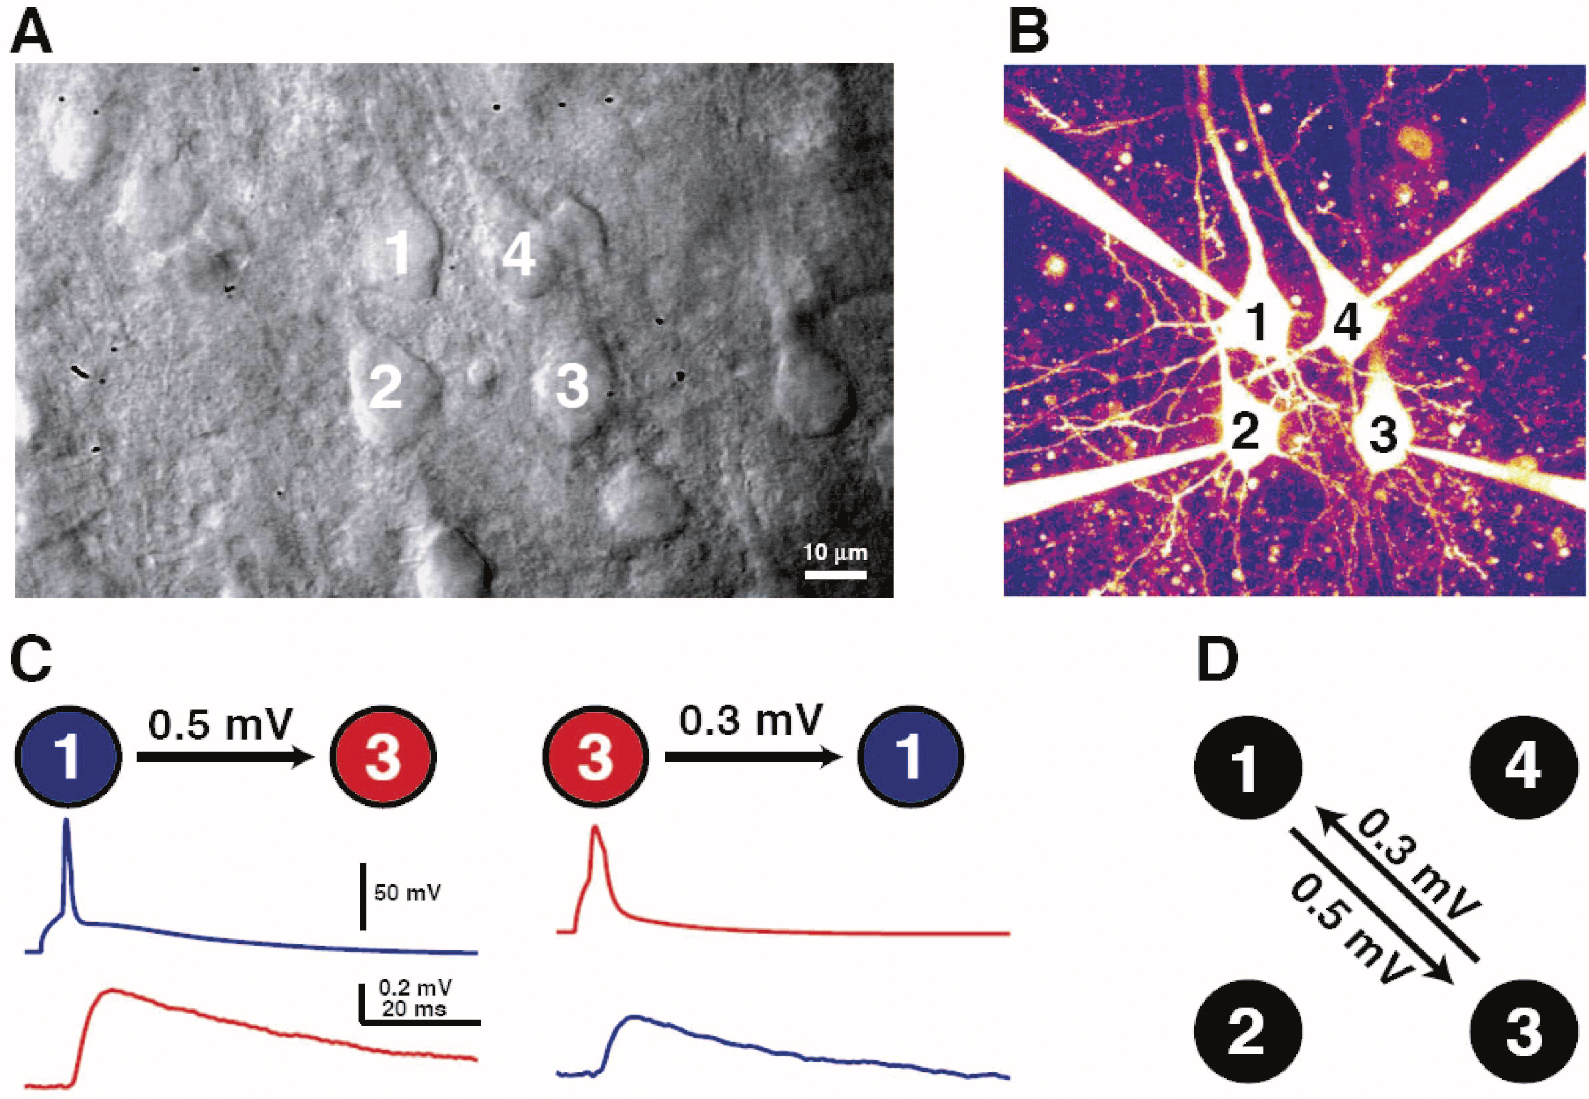
\includegraphics[width=.75\linewidth]{img/song2005-quadruplet_recordings.png}
%   \caption{Song et al. use quadruple whole-cell recordings, observing
%     simultaneously the membrane potential of four neurons.
%     \textbf{A)} Contrast image showing four thick-tufted L5 neurons
%     \textbf{B)} Fluorescent image of the same cells after patching on
%     \textbf{C)} Evoking an action potential in the presynaptic neuron
%     causes characteristic membrane potential change in the
%     postsynaptic neuron \textbf{D)} Infering synaptic connectivity
%     from the EPSP waveform observed in C). Image from \parencite{Song2005}.
%     % \texttt{\textcolor{linkgrey}{3b056efe-3ebc}}
%   }
% \end{figure}
% \vspace{0.45cm}

% While techniques for paired intracellular recordings are rapidly
% developing, their ability to capture connectivity patterns of large
% networks is yet very limited. To this date, the connectome of
% \textit{C. Elegans} remains the outstanding exception of a
% connectivity configuration that has been fully mapped
% [\textcolor{linkgrey}{Source}]%??
% . Even in the state-of-the-art experiment conducted by Perin et al.,
% using a setup capable of recording up to twelve neurons
% simultaneously, the authors note that an investigation of degree
% distribution was not carried out, due to lack of sufficient data
% \parencite{Perin2011}.

% \subsection*{Exploiting the benefits of a geometrical model}

% Working with a geometrical network model and its computational
% implementation, such restrictions disappear; the full information
% about the network, in form of its connectivity matrix, is given at
% point in time and can be easily queried for. Experiments that may take
% days to perform \textit{in vivo}, can be completed in a matter of seconds \textit{in
% silico}. As such, geometrical models lend themselves to extensive
% examination of their structural aspects.

% In trying to exploit these advantages, two approaches present
% themselves. One may construct a network model that
% extrapolates\graffito{Extrapolation vs. reduction} the known
% biological configuration; a full structural examination of these
% networks could possibly expose relevant patterns not yet observed. For
% this approach a sophisticated understanding of the biological
% configuration is critical. Neuron morphology, however, is difficult to
% describe and extract.

% For this analysis we suggest a reductionist approach. Having motivated
% an abstract model reflecting a cortical network's directional
% heterogeneity, we distinguish emerging patterns of connectivity,
% specific to directionally heterogeneous networks, from results, that
% only indirectly stem from the network's anisotropy, in the hopes to be
% able to characterize the significance of directional heterogeneity in
% structural connectivity of cortical circuits.


% \subsection*{Structural aspects of the heterogeneous model}

% In this chapter we subject the anisotropic network
% model introduced in Section~\ref{sec:anisotropic_network_model} to a
% critical analysis of its structural aspects. General network topology,
% as well as specific modes and patterns of connectivity, are to be
% identified and laid out for comparison with findings in biological
% neural networks.

% In an effort to map out structural features that can be directly
% associated with the network's directional \marginpar{employing
%   anisotropy measure} heterogeneity, it is crucial to differentiate
% such findings from results that are only indirectly caused by the
% network's anisotropy. To this end, already in
% Section~\ref{sec:anisotropy_measure} we developed a measure to
% quantify the degree of anisotropy prevalent in a given network;
% throughout this chapter we will now frequently employ this measure to
% determine which structural aspects are originating from the network's
% heterogeneity, and which aspects are to be attributed solely to the
% network's distance dependency.

% Accordingly, results from this investigation are categorized in two
% sections: The first section, 'Section 2' %??
% , describes structural aspects that can not be directly attributed to
% the model's anisotropy. The second section, 'Section 3' %??
% , then presents results that are truly features of network's
% directional heterogeneity.


% ######################################################################### %
% ------------------------------------------------------------------------- %
%                             Comment Stuff
% ------------------------------------------------------------------------- %
% ######################################################################### %


% Human Connectome Project and the Open Connectome Project, the
% continued development of experimental techniques and of resources
% like the Brain Connectivity Toolbox software, as well as the
% research of theoreticians and experimentalists, are all dedicated
% towards the common goal of charting brain connectivity.

% In this general sense, brain connectivity can refer to linking
% between distinct units at various scales. From the mapping of fiber
% pathways between brain regions on the macroscale, to the synaptic
% connections of individual neurons on the microscale,
% [\textcolor{linkgrey}{Scholarpedia}].

% It is interesting not only to investigate for anatomical
% connections, but functional and causal as well. However, exploring
% the aspects of our specific geometric network model, in this chapter
% the connectivity of interest to us is the structural connectivity at
% the microscale, that is synaptic connections between individual
% neurons.

% \marginpar{Human Connectome Project
% \mbox{\url{humanconnectome.org}}}

% \parbox{1.8cm}{Human Connectome
% Project}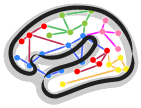
\includegraphics[width=0.45\linewidth]{img/HCP_logo.png}
% \mbox{\url{humanconnectome.org}}}


% Ho Ko connectivity -> specific dynamics.
% Pernice -> Spike Train Correlations. Maybe Shepherd 2005?

% ...and have been linked to brain function and dynamics.

% *What cool things synaptic connectivity does.  , stores memory, drives
% dynamics, etc.  While brain is plastic, there is structure that is
% believed to provide a framework, boundary conditions to

% *patterns of synaptic connectivity is neither completely random nor
% exclusively specific, patterns emerge [Sporns, Perin, Song]
 
% This specific, non-random connectivity largely impact dynamics and
% brain function:


% Connectivity in the directionally heterogenous geometric networks
% introduced in ??, models synaptic contacts between axon and
% dendrites of individual neurons. In this chapter

% It is then the task of this theoretical framework to provide results
% interesting to the biological situation. An investigation on how well
% an introduced model can reproduce certain structural aspects of
% networks that have already been fund is integral to the study of a
% computational model. But, furthermore, a model should aspire to
% extrapolate results found in the biological
% situation.





% ######################################################################### %
% ------------------------------------------------------------------------- %
%                     Degree distribution
% ------------------------------------------------------------------------- %
% ######################################################################### %

% \section{Degree distribution}\label{sec:degree_distribution}

% The in- and out-degree of vertex in a directed graph describes the
% number of incoming and outgoing connection from and to other vertices
% (cf. Definition~\ref{def:in_out_degree}). As a fundamental concept in
% graph and network theory, the degree distribution is integral in the
% categorization of networks and allows for the estimation of graph
% properties.

% Degree distribution was shown to have strong impact on the dynamics of
% neuronal networks models commonly used in computational neuroscience
% research \parencite{Roxin2011}. Increasing in-degree variance for
% example could be connected to the appearance of oscillations in the
% network. Extracting degree distributions from biological networks
% however, remains a challenge as many neurons need to be tracked
% simultaneously to obtain enough data to confidently estimate degree
% distributions. 

% \begin{figure}[H]
%   \centering
%   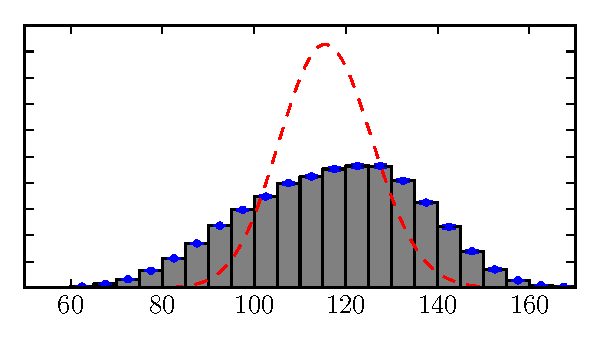
\includegraphics[width=0.7\textwidth]{%
%     plots/9326138e.pdf}
%   \caption{\textbf{In-degree distribution in anisotropic networks
%       shows comparably high variance and is skewed to the left} From 250
%     anisotropic networks in-degree distributions were extracted and
%     are shown in a normed histogram plot, errorbars SEM. Comparison with the
%     binomial degree distribution (red) of a Gilbert random graph model
%     with matching parameter set ($N=1000$, $p =0.116$) shows higher
%     variance of in-degrees in anisotropic networks (sample variance $=
%     344.54$, variance of binomial distribution $Np(1-p) = 102.44$.)
%     Skewness to the left of the sample is $-0.1763.$
%     (\smtcite{9326138e})}
%   \label{fig:in_degree_ER_compare}
% \end{figure}

% Here we analyze in- and out-degrees in the anisotropic network
% model. First we find that compared to the binomial in-degree
% distribution of a Gilbert random graph model, in-degrees of vertices
% in anisotropic networks display higher variance and their distribution
% is skewed to the left (\autoref{fig:in_degree_ER_compare}). However,
% this specific in-degree profile is not an intrinsic property of
% anisotropy, as the distribution remains stable under manipulation of
% the anisotropy degree and closely matches the profile of a purely
% distance-dependent network (\autoref{fig:in_degree_rewiring}). This
% result agrees with findings of \textcite[Fig. S3]{Perin2011}, who were
% able to recreate degree distributions from their experiment with layer
% V thick-tufted pyramidal cells in neonatal rats from the extracted
% distance-dependent connection profiles alone.



% \begin{figure}[H]
%   \centering
%   \renewcommand{\tabcolsep}{2pt}
%   \setlength\extrarowheight{0pt}
%   \begin{tabular}{lll}
%     \begin{overpic}[width=0.28\textwidth]{%
%         plots/77995b6b_in000.pdf}
%       \put(12,56){\small $\eta = 0$}
%     \end{overpic}
%     &
%     \begin{overpic}[width=0.28\textwidth]{%
%         plots/77995b6b_in025.pdf}
%       \put(12,56){\small $\eta = 0.25$}
%     \end{overpic}
%     &
%     \begin{overpic}[width=0.28\textwidth]{%
%         plots/77995b6b_in050.pdf}
%       \put(12,56){\small $\eta = 0.5$}
%     \end{overpic}
%     \\
%     \begin{overpic}[width=0.28\textwidth]{%
%         plots/77995b6b_in075.pdf}
%       \put(12,56){\small $\eta = 0.75$}
%       \put(4,-4){\small$0$}\put(78,-4){\small$200$}
%     \end{overpic}
%     &
%     \begin{overpic}[width=0.28\textwidth]{%
%         plots/77995b6b_in100.pdf}
%       \put(12,56){\small $\eta = 1$}
%       \put(4,-4){\small$0$}\put(78,-4){\small$200$}
%     \end{overpic}
%     & 
%     \begin{overpic}[width=0.28\textwidth]{%
%         plots/77995b6b_indst.pdf}
%       \put(12,56){\small distance}
%       \put(4,-4){\small$0$}\put(78,-4){\small$200$}
%     \end{overpic}
%     \\
%   \end{tabular}
%   \caption{\textbf{In-degree distribution not affected by varying
%       degrees of anisotropy} In-degree distributions from the 25
%     sample graphs (ref ??) and their rewiring stages are plotted in
%     normed histograms and listed from rewiring factor $\eta =0$
%     (original anisotropic) to $\eta = 1$ (completely rewired, maximal
%     isotropy). Comparison shows that varying degrees of anisotropy do
%     not influence the degree distribution, in fact in-degree
%     distributions match with the degree distribution of an equivalent
%     distance-dependent network shown bottom-right (\smtcite{77995b6b}). }
%   \label{fig:in_degree_rewiring}
% \end{figure}


% While the out-degree distribution of vertices in the anisotropic
% network also shows itself stable under rewiring, its distribution is
% drastically different from the out-degree distribution in a comparable
% distance-dependent network (\autoref{fig:out_degree_rewiring}). The
% asymmetric, long-tailed distribution is identified as an artifact of
% the anisotropic network's spatial confinement; a neuron, closely
% located near a surface edge, might have an axon projection out of the
% square causing minimal out-degree or, projecting through the entire
% length of the surface, may have maximal out-degree. Approximating the
% expected number of outgoing connections for a vertex in an anisotropic
% network of size $N$, side-length $s$ and axon width $w$ as
% \[
%   N \frac{w l}{s^2},
% \]
% with parameters $N = 1000$ and $\frac{w}{s} = 0.252$, we obtain an
% upper bound for the expected out-degree, 
% \[
%   N \frac{w l}{s^2} \leq N\frac{w}{s} \sqrt{2} \approx 350.
% \]
% If $f(l)$ is the probability density function to find axon length $l$
% for a random node $v$ in the anisotropic network model, the out-degree
% distribution is then approximated by
% %
% \begin{align}\label{eq:axon_length_approx}
%   \mathbf{Pr}[d_{\mathrm{out}}(v) = N \frac{w l}{s^2}] = f(l),  
% \end{align}
% %
% see also \autoref{fig:out_degree_ER_compare}.

% \begin{figure}[H]
%   \centering
%   \renewcommand{\tabcolsep}{2pt}
%   \setlength\extrarowheight{0pt}
%   \begin{tabular}{lll}
%     \begin{overpic}[width=0.28\textwidth]{%
%         plots/77995b6b_out000.pdf}
%       \put(12,56){\small $\eta = 0$}
%     \end{overpic}
%     &
%     \begin{overpic}[width=0.28\textwidth]{%
%         plots/77995b6b_out025.pdf}
%       \put(12,56){\small $\eta = 0.25$}
%     \end{overpic}
%     &
%     \begin{overpic}[width=0.28\textwidth]{%
%         plots/77995b6b_out050.pdf}
%       \put(12,56){\small $\eta = 0.5$}
%     \end{overpic}
%     \\
%     \begin{overpic}[width=0.28\textwidth]{%
%         plots/77995b6b_out075.pdf}
%       \put(12,56){\small $\eta = 0.75$}
%       \put(4,-4){\small$0$}\put(78,-4){\small$350$}
%     \end{overpic}
%     &
%     \begin{overpic}[width=0.28\textwidth]{%
%         plots/77995b6b_out100.pdf}
%       \put(12,56){\small $\eta = 1$}
%       \put(4,-4){\small$0$}\put(78,-4){\small$350$}
%     \end{overpic}
%     & 
%     \begin{overpic}[width=0.28\textwidth]{%
%         plots/77995b6b_outdst.pdf}
%       \put(52,56){\small distance}
%       \put(4,-4){\small$0$}\put(78,-4){\small$350$}
%     \end{overpic}
%     \\
%   \end{tabular}
%   \caption{\textbf{Out-degree distribution not affected by varying
%       anisotropy but highly different from distance-dependent
%       networks} Out-degree distributions from the 25 sample graphs
%     (ref ??) and their rewiring stages are plotted in normed
%     histograms and listed from rewiring factor $\eta =0$ (original
%     anisotropic) to $\eta = 1$ (completely rewired, maximal
%     isotropy). While varying degrees of anisotropy do not influence
%     the degree distribution, the characteristic out-degree profile is
%     drastically different from the distribution found in equivalent
%     distance-dependent networks (\smtcite{77995b6b}). }
%   \label{fig:out_degree_rewiring}
% \end{figure}



% \begin{figure}[H]
%   \centering
%   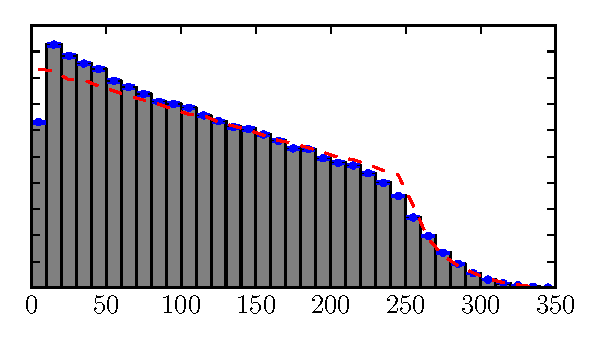
\includegraphics[width=0.7\textwidth]{%
%     plots/019555b0.pdf}
%   \caption{\textbf{Characteristic out-degree distribution as an
%       artifact of network's boundaries} From 250 anisotropic networks
%     out-degree distributions were extracted and are shown in a normed
%     histogram plot, errorbars SEM. The characteristic distribution is
%     identified as an artifact of the network's spatial confinement;
%     using equation~\ref{eq:axon_length_approx} the out-degree profile
%     is approximated (red) by the distribution of axon lengths in the
%     anisotropic network (\smtcite{019555b0}).}
%   \label{fig:out_degree_ER_compare}
% \end{figure}
% %------------------------------------------------
% \marginpar{\vspace{-8.1cm}\\Steep incline for small out-degree cut off
%   due to binning (cf. \autoref{suppfig:out_degree})} 
% %------------------------------------------------




% ######################################################################### %
% ------------------------------------------------------------------------- %
%                        Small World Properties
% ------------------------------------------------------------------------- %
% ######################################################################### %


\section{Small World Properties}

Sporns papers



\section{Motifs}




%%% Local Variables: 
%%% mode: latex
%%% TeX-master: "../dplths_document"
%%% End: 
